\clearpage
\section{hardness of the problem}
\label{PCQharness}

\subsection{Preliminaries}
\begin{definition}[$\#$P~\cite{valiant}]
A counting problem that can be computed by nondeterministic Turing machine running in polynomial time is categorised in the class $\#$P.
\end{definition}

\begin{definition}[$\#$P-hard~\cite{valiant}]
A problem is $\#$P-hard if all problems in $\#$P reduce to it. 
\end{definition}

\begin{definition}[$\#$P-complete~\cite{valiant}]
A problem is $\#$P-complete if all problems in $\#$P reduce to it and it belongs to $\#$P. 
\end{definition}

In computational complexity theory and computability theory, a counting problem is a problem only returns the number of all solutions and it is $\#P$. Valiant further defined the class $\#$P-complete as the ``hardest" problem in $\#$P as the concept of NP-complete is introduced in NP problems. Garey et al.~\cite{garey1979guide} and Papadimitriou et al.~\cite{papadimitriou2003computational} proved that if a counting problem is $\#$P-complete, then its associated problem of mining all solutions must be NP-hard. Based on above conclusion, GuiZhen Yang has proved that mining frequent itemsets including subtrees is NP-hard~\cite{yang2004complexity}. As for our problem which holds three property defined in Problem~\ref{PCQ}, all validated communities are required to computed. Thus we follow the same principle that if we can prove that (in worst case) counting the number of all required communities is $\#$P-complete, then our problem is NP-hard. 

{\bf Bipartite graph.}
A bipartite graph can be denoted as a triple, $G=(U,V,E)$, where vertices can be partitioned to two disjoint sets $U$ and $V$, and $E$ is the set of edges between vertices in $U$ and $V$, i.e., $E\subseteq U\times V$.  

A bipartite clique is a subgraph of a bipartite graph such that every vertices in two distinct vertex sets are adjacent. Furthermore, a bipartite clique $G'=(U',V',E')$ is a maximal bipartite clique in a given bipartite graph, if there exists no other bipartite clique $G''=(U'',V'',E'')$ such that $U'\subseteq U''$, $V'\subseteq V''$, $E'\subseteq E''$ simultaneously. 

{\bf Construction of bipartite graph.}
Since each node in P-tree is unique and has fixed location in P-tree, knowing all p-tree nodes is enough to reconstruct the original P-tree. Then we can simply construct a bipartite graph $G=(U,V,E)$ from the profiled graph where $U$ is the set of all users in the profiled graph and $V$ is the set of all unique P-tree nodes. Edges in $E$ represent that users in $U$ own the P-tree nodes in $V$. The construction process can be done in linear time. Note that this constructed bipartite graph is not equivalent to the associated profiled graph, because connectiveity of vertices in the profiled graph is not presented in $G=(U,V,E)$. But in the case that the profiled graph is a complete graph which means each induced subgraph is a clique, the profiled graph can be constructed to a bipartite graph without losing generality. 

Based on the assumption and this one-to-one correspondence, we can reduce the problem of computing the number of all maximal bipartite cliques containing query node $q$ in the bipartite graph to the problem of computing the number of required communities with $q$ in the profiled graph. The former one is shown in Theorem~\ref{bipartiteclique}, then the latter one will be proved $\#$P-complete.

\subsection{Proof}
 \begin{theorem}[~\cite{provan1983complexity}]
\label{bipartiteclique}
The problem of counting the number of maiximal bipartite cliques in a given bipartite graph is $\#$P-complete.
\end{theorem}

Let $C_i(G)$ denote a set of all qualified communities and $\forall C \in C_i(G)$, $|C|=i$; $M_i(G)$ represents a set of all qualified communities and $\forall M \in M_i(G)$, $|M|\geq i$. Clearly, $M_k(G)$ is the set of all targeted communities which hold the problem definitions.
Based on Theorem~\ref{bipartiteclique}, we have Corollary~\ref{countingPCQ}. 

\begin{corollary}
\label{countingPCQ}
It is $\#$P-complete to counting the $\sum_{i=1}^{|G|}{|C_i(G)|}$.
\end{corollary}

Now we construct a new bipartite graph followed the strategy in \cite{yang2004complexity} and represent it as a binary martix. 
Since the required community contains $q$, the maxinum common subtree of the community must be the subtree of $q$'s. Let $V=\{v_1,v_2,...,v_n\}$ be the set of $q$'s P-tree nodes and $U=\{u_1,u_2,...,u_m\}$ be all vertices in the profiled graph. $D$ denotes the database which recording the relationship between $U$ and corresponding tree nodes $V$. Note that the construcution of $D$ can be done from the original profiled graph in polynomial time. Then, we generate $m$ new items namely $L=\{l_1,l_2,...,l_m\}$ and $m$ new vertices $S=\{s_1,s_2,...,s_m\}$. Let function $w$ denote expanded items of the vertex in $U^+$. As shown in Figures~\ref{fig:newMatrix}, the new bipartite graph $D^+$ is constructed as follows: 

(1). $U^+=U \cup S$. 

(2). For $i\in [1,m], W(u_i)=D_i \cup L, W(s_i)=V \cup (L-{l_i})$. 

\begin{figure}
	\centering
	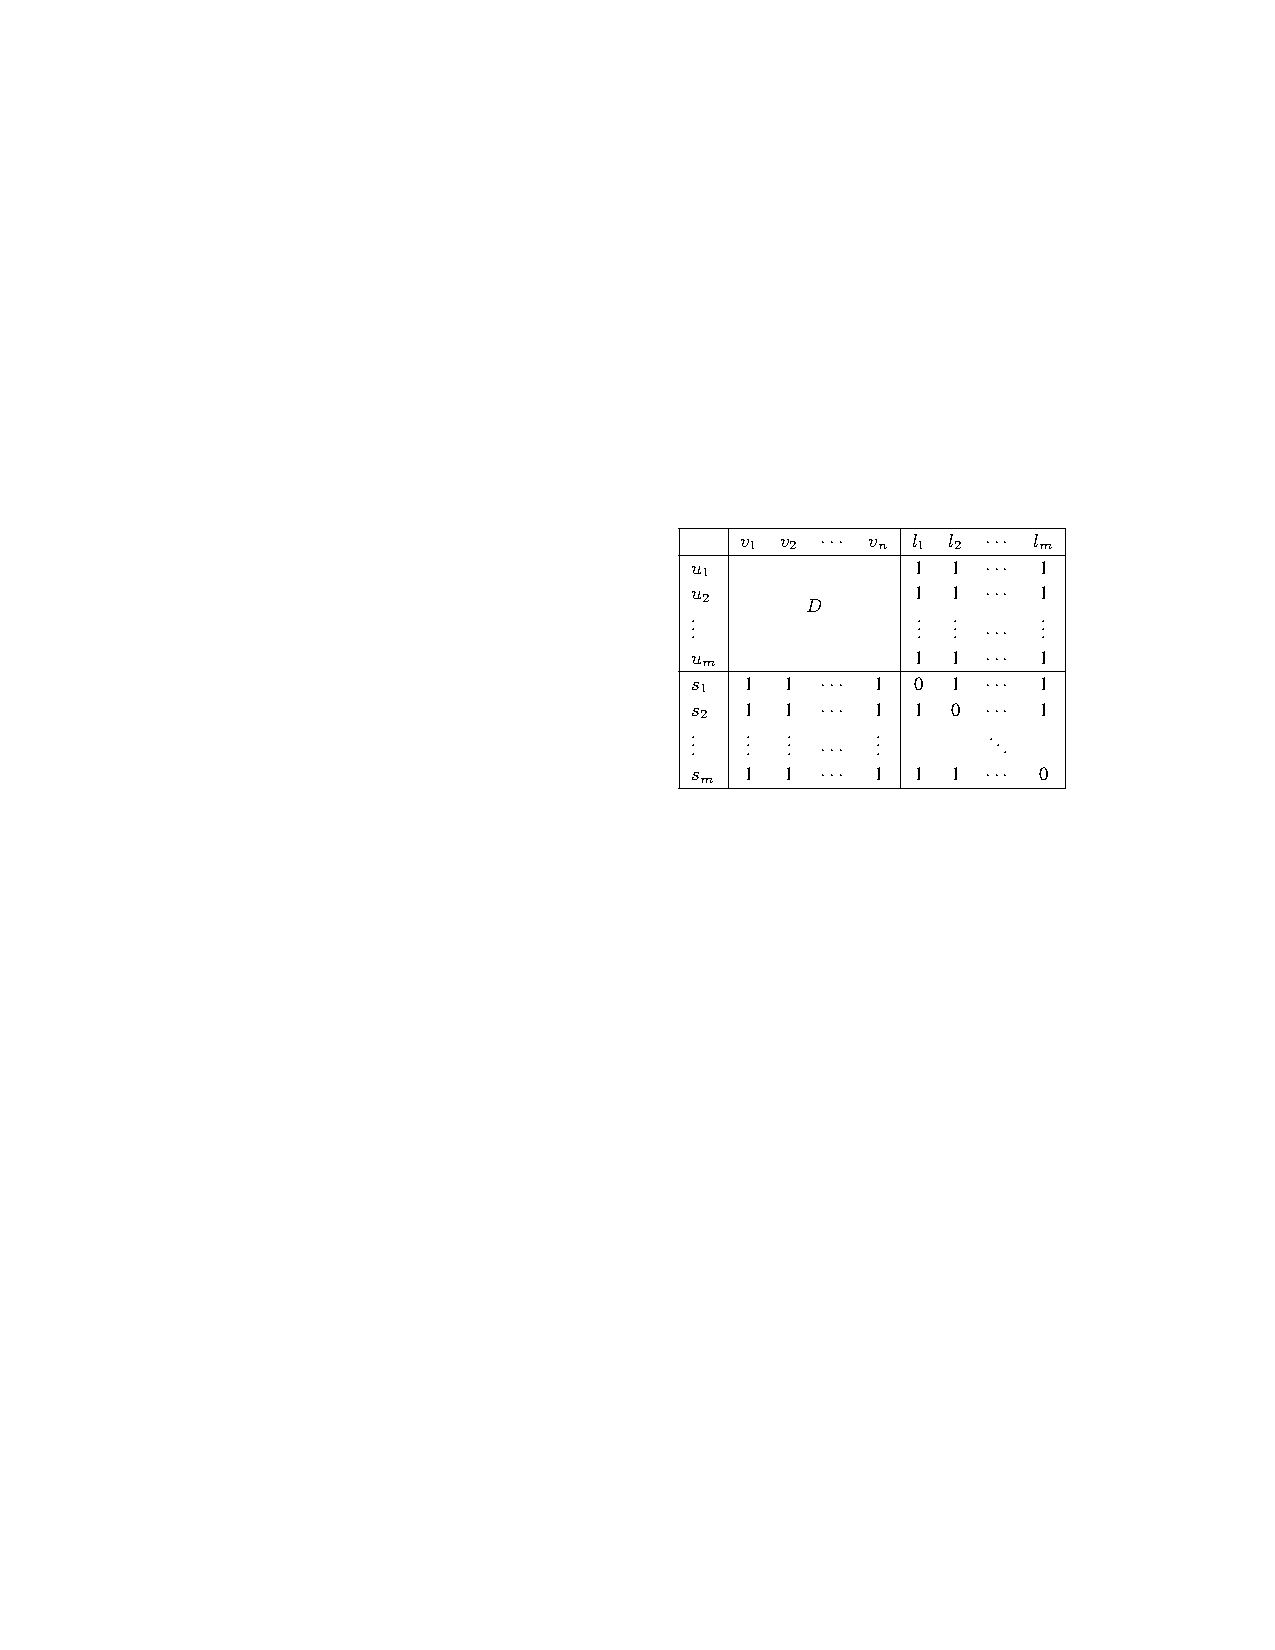
\includegraphics[width=0.88\linewidth]{Figures/ExpandMatrix}
	\caption{Binary matrix representation of bipartite graph $D^+$.}
	\label{fig:newMatrix}
\end{figure} 


\iffalse
\begin{tabular}{|l|cccc|cccc|l|}
\hline
&$v_1$ & $v_2$ & $\cdots$ & $v_n$ & $l_1$ & $l_2$ & $\cdots$ & $l_m$ \\
\hline
$u_1$ 	 & \multicolumn{4}{c|}{\multirow{4}*{{$D$}}}		&    1	   &     1	  & $\cdots$ &     1    \\
$u_2$ 	 &&&&												&    1 	   &     1	  & $\cdots$ &     1    \\
$\vdots$ &&&&												& $\vdots$ & $\vdots$ & $\cdots$ & $\vdots$ \\
$u_m$ 	 &&&&												&    1 	   &     1	  & $\cdots$ &     1    \\
\hline
$s_1$ 		&	   1	  &     1	  & $\cdots$ &     1	&    0	   &     1	  & $\cdots$ &     1    \\
$s_2$ 		&	   1	  &     1	  & $\cdots$ &     1	&    1 	   &     0	  & $\cdots$ &     1    \\
$\vdots$ 	&  $\vdots$   & $\vdots$  & $\cdots$ & $\vdots$ & 		   & 		  & $\ddots$ &  		\\
$s_m$ 		&      1	  &     1	  & $\cdots$ &     1	&    1 	   &     1	  & $\cdots$ &     0    \\
\hline
\end{tabular}
\fi


\begin{lemma}
\label{expandGraph}
$\forall a \in [0,m-\sigma]$, if a commmunity in $C_{\sigma +a}(G)$ whose maximum common subtree is $I$, $\sigma \in [1,m]$, then for any arbitrary itemset $L_a \subseteq L$, $|L_a|=a$, there must exist an communitiy in $C_{\sigma +m}(D^+)$ such that $I \cup L_a$ is its maximum common subtree. 
\end{lemma}  

\begin{proof}
If $I$ is the maximum common subtree of a community in $C_{\sigma +a}(G)$, which means $I$ is shared by $\sigma +a$ vertices ranging from $u_1$ to $u_m$. Then $I \cup L_a$ is still shared by these vertices because $L_a \subseteq L$. As for vertices from $s_1$ to $s_m$, $I$ is shared by all of them. Note that $W(s_i)=V \cup (L-{l_i})$ and $|L_a|=a$, thus there are $m-a$ vertices from $s_1$ to $s_m$ that do not contains all items in $L_a$. In conclusion, for any any arbitrary itemset $L_a$, $I \cup L_a$ is shared by $\sigma +m$ vertices in $D^+$ which means these vertices group a community whose maximal common subtree is $I \cup L_a$.
\end{proof}

\begin{lemma}
\label{MC}
$M_{\sigma +m}(D^+)$ = $C_{\sigma +m}(D^+)$
\end{lemma}

Lemma~\ref{MC} implies that if there is a community in $C_{\sigma +m}(D^+)$ whose maximum common subtree is $I'$ iff if there exists a community in $M_{\sigma +m}(D^+)$ whose maximum common subtree is $I'$ as well. 

\begin{proof}
We prove necessity of Lemma~\ref{MC} first and sufficiency follows.

$\bullet$ \textbf{Necessity.} It is obvious from the definition.

$\bullet$ \textbf{Sufficiency.} $I'$ can be constructed as $I'= I \cup L_a$, where $L_a$ is an arbitrary itemset and $|L_a|=a$. Since $I'$ is shared by at least $\sigma +m$ vertices in $D^+$ and $I'$ is shared by $m-a$ vertices from $s_1$ to $s_m$, $I'$ is shared by at least $\sigma+a$ vertices from $u_1$ to $u_m$ which group a community in $D$ as well. From Lemma~\ref{expandGraph}, if $I'$ is shared by $\sigma+a' (a'>a)$ vertices in $D$, $I'$ will be shared by $\sigma+m$ vertices in $D^+$ which means there exists a community in $C_{\sigma +m}(D^+)$ sharing $I'$. That proves the necessity part. 
\end{proof}

Based on Lemma~\ref{MC}, we have the following equation.

\begin{lemma}
\label{equation}
Let $D$ denote the original database and $D^+$ be the expanded database, $|U|=m$, for $\sigma \in [1,m]$:

$|M_{\sigma +m}(D^+)| = \displaystyle{\sum_{a=0}^{m-\sigma}}|C_{\sigma +a}(D)| \cdot \binom{m}{a}$.
\end{lemma}

\begin{theorem}
$G={U,V}$ denotes the profiled graph, $|U|=m$, the problem of computing $|M_k(G)|$ where $k \in [1,m]$, is $\#P$-complete.
\end{theorem}


\begin{proof}
Checking whether a community is satisfying all properties or not can be done in polynomial time. Therefore, the problem of computing $|M_k(G)|$ is in $\#$P. We now reduce the problem of counting the number of $\sum_{i=1}^{|G|}{|C_i(G)|}$ as stated in Corollary~\ref{countingPCQ} to the problem of the counting of computing $|M_k(G)|$, thereby proving that the latter one is $\#$P-hard.

First, we can construct $D$ from the orginal profiled graph $G$ in polynomial time. Let $C_\sigma =C_{\sigma}(D)$, $M_\sigma=M_{\sigma+m}(D^+), \sigma \in [1,m]$. Based on Lemma~\ref{equation}, we have following linear equtions. 

$$
\left[
\begin{matrix}
C_1 \\ C_2 \\C_3 \\\vdots\\ C_m
\end{matrix}
\right]=\\
\left[
\begin{matrix}
 \binom{m}{0}  & \binom{m}{1} & \binom{m}{2} & \cdots & \binom{m}{m-1}     \\
 0 			   & \binom{m}{0} & \binom{m}{1} & \cdots & \binom{m}{m-2}     \\
 0 			   & 0            & \binom{m}{0} & \cdots & \binom{m}{m-3}     \\
 			   & 			  &				   \ddots				   	   \\
 0 			   & 0            & 0			 & \cdots & \binom{m}{m-(m-1)} \\
\end{matrix}
\right]^{-1} \\
\cdot \\
\left[
\begin{matrix}
M_1 \\ M_2 \\M_3 \\\vdots\\ M_m
\end{matrix}
\right]
$$


If we have a polynomial-time algorithm for computing $|M_k(G)|$, we can compute $(M_1,M_2,\cdots,M_m)$ in polynomial time. Since $ \forall x \in [0,m-1], \binom{m}{x}$ can be compute in O(m), $(C_1,C_2,\cdots,C_m)$ and $\sum_{\sigma=1}^{m}{C_\sigma}$ can be computed in polynomial time and therefore the problem of computing the number of $|M_k(G)|$ is $\#$P-complete.    
\end{proof}

In conclusion, since the problem of counting the number of all qualified communities is $\#$P-complete, the problem of mining all PCQ communities is NP-hard.



